\documentclass[utf8, a4paper, 14pt, russian, oneside]{book}

% Размер шрифта
\usepackage[14pt]{extsizes}

% Кодировка
\usepackage[T2A]{fontenc}
\usepackage[utf8]{inputenc}
\usepackage[main=russian, english]{babel}

\usepackage{fontspec}
\setmainfont{Times New Roman}
\usepackage{sectsty}
\sectionfont{\large}
\subsectionfont{\large}

% Параметры страницы
\usepackage[left=3cm, right=1cm, top=2cm, bottom=2cm]{geometry}
\pagestyle{plain}
\linespread{1.1} % Межстрочный интервал

% Пакеты для работы с математикой
\usepackage{amsmath}
\usepackage{amsfonts}
\usepackage{amssymb}

% Вставка изображений
\usepackage{graphicx}

% Пакет для работы с таблицами
\usepackage{tabularx}
\usepackage{booktabs}
\usepackage{longtable}

% Для больших множеств
\usepackage{mathtools}

% Для работы с рисунками
\usepackage{caption}

% Для создания графов в 3 блоке
\usepackage[all]{xy}

% Для специальных символов
\usepackage{textcomp}

% Для гиперссылок
\usepackage{hyperref}

% Для таблиц
\usepackage{multirow}

\usepackage{upgreek}

\usepackage{array}
\newcommand{\mysec}[1]{
{\centering\section*{\hyperlink{toc}{#1}}}
\addcontentsline{toc}{section}{#1}
}

\newcommand{\mysubsec}[1]{
{\centering\subsection*{\hyperlink{toc}{#1}}}
\addcontentsline{toc}{subsection}{#1}
}

\newcommand{\Db}{
    \ensuremath{
        D_{\text{в}}
    }
}

\newcommand{\xb}{
    \ensuremath{
        x_{\text{в}}
    }
}

\newcommand{\yb}{
    \ensuremath{
        y_{\text{в}}
    }
}

\newcommand{\zb}{
    \ensuremath{
        z_{\text{в}}
    }
}

\newcommand{\yx}{
    \ensuremath{
        y_x
    }
}

\newcommand{\zx}{
    \ensuremath{
        z_x
    }
}

\newcommand{\cov}{
    \ensuremath{
        \mathit{cov}_{\text{в}}
    }
}

\renewcommand{\r}{
    \ensuremath{
        \mathit{r}_{\text{в}}
    }
}

\newcommand{\rang}{
    \ensuremath{
        \mathit{rang}
    }
}

\newcommand{\rhob}{
    \ensuremath{
        \rho_{\text{в}}
    }
}

\newcommand{\der}[2]{
    \ensuremath{
        \frac{\partial #1}{\partial #2}
    }
}

% Команды для настройки содержания
\renewcommand\contentsname{\center{Содержание}} % Вместо оглавления пишется содержание
\addto{\captionsenglish}{\renewcommand{\bibname}{References}}
\begin{document}

\thispagestyle{empty}
~\vspace{-2cm}\setlength{\parindent}{0cm}
\begin{center}
	
\includegraphics[scale=1.5]{../include/logo.png}\\[2pt]
	МИНОБРНАУКИ РОССИИ\\
	Федеральное государственное бюджетное образовательное учреждение\\
	высшего профессионального образования\\[5pt]
	\textbf{<<МИРЭА – Российский технологический университет>>}\\[5pt]
	\textbf{\large РТУ МИРЭА}\\[20pt]
	\hrule{}\mbox{}\\[1pt]
	\hrule{}\mbox{}\\[20pt]	
	Институт кибернетики \\ Кафедра <<Информационная безопасность>> (БК №252)\\[35pt]
	\textbf{Долгосрочное задание} \\
	по дисциплине: Математическая статистика
\end{center}
	\vspace{4in}
	Студент группы ККСО-01-19:  \qquad \qquad \qquad  \qquad     Колесников А.В.
\vspace{0.6in}
\begin{center}
Москва --- 2021
\end{center}
\newpage

\tableofcontents
\newpage

\mysec{Описание данных}

В качестве данных возьмем данные о цене на курс криптовалюты <<Ethereum>> (в долларах) в период времени с 8 ноября по 7 декабря. Объём выборки равен 30.
Пусть X - цена криптовалюты.
\begin{table}[h!]
    \centering
    \begin{tabular}{|c|c|c|}
        \hline
        № & Дата & Цена \\ \hline
        1 & 11.08 & 4619,65 \\ \hline
        2 & 11.09 & 4810,07 \\ \hline
        3 & 11.10 & 4733,36 \\ \hline
        4 & 11.11 & 4635,45 \\ \hline
        5 & 11.12 & 4724,31 \\ \hline
        6 & 11.13 & 4666,72 \\ \hline
        7 & 11.14 & 4648,63 \\ \hline
        8 & 11.15 & 4627,09 \\ \hline
        9 & 11.16 & 4570,48 \\ \hline
        10 & 11.17 & 4213,91 \\ \hline
        11 & 11.18 & 4287,80 \\ \hline
        12 & 11.19 & 3995,73 \\ \hline
        13 & 11.20 & 4298,35 \\ \hline
        14 & 11.21 & 4412,20 \\ \hline
        15 & 11.22 & 4266,51 \\ \hline
        16 & 11.23 & 4089,68 \\ \hline
        17 & 11.24 & 4340,04 \\ \hline
        18 & 11.25 & 4271,39 \\ \hline
        19 & 11.26 & 4522,21 \\ \hline
        20 & 11.27 & 4043,00 \\ \hline
        21 & 11.28 & 4101,65 \\ \hline
        22 & 11.29 & 4296,95 \\ \hline
        23 & 11.30 & 4447,77 \\ \hline
        24 & 12.01 & 4623.68 \\ \hline
        25 & 12.02 & 4586,33 \\ \hline
        26 & 12.03 & 4514,36 \\ \hline
        27 & 12.04 & 4227,76 \\ \hline
        28 & 12.05 & 4119,63 \\ \hline
        29 & 12.06 & 4199,00 \\ \hline
        30 & 12.07 & 4369,08 \\ \hline
    \end{tabular}
\end{table}
\newpage

\mysec{График динамики ряда}
Временной ряд - это собранный в разные моменты времени статистический материал о значении каких-либо параметров.

\begin{figure}[h!]
    \centering
    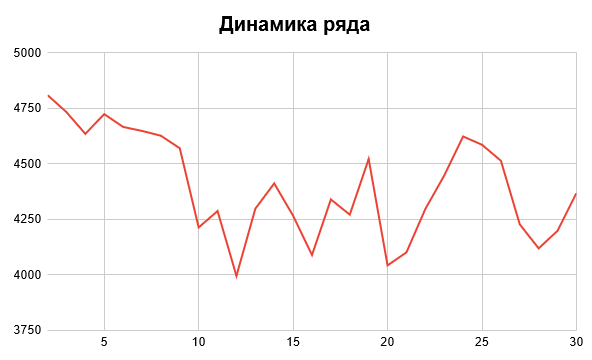
\includegraphics{img/dynamic_range.png}
    \caption{Динамика ряда.}
\end{figure}

\mysec{Автокорреляционная функция}
Автокорреляция - это обычный коэффициент корреляции для значений одной величины в разные моменты времени (лаги).
Серию коэффициентов автокорреляции уровней ряда с последовательным увеличением величины лага принято называть автокорреляционной функцией.
Автокорреляция в момент вермени $k$ вычисляется по следующей формуле:
\begin{gather*}
    r(k) = \frac{\cov(X, Y)}{\sqrt{\Db(X)}\sqrt{\Db(Y)}}
    = \frac{
        \overline{x_k \cdot x_{k-1}} - \overline{x_k} \cdot \overline{x_{k-1}}
    }{
        \sigma_k \cdot \sigma_{k-1}
    }
\end{gather*}

Если $X = \{ x_1, \ldots, x_{30} \}$, то $X_k = \{ x_1, \ldots, x_{n-k} \}, X_{k-1} = \{ x_{1+k}, \ldots, x_n \}, k \in \overline{1, \tfrac{n}{2}}, m = n - k$.

Найдём $r(1)$. Для этого необходимо вычислить вспомогательные значения:
\begin{gather*}
    X_1 = \{x_1, \ldots, x_{29}\} \qquad X_2 = \{x_2, \ldots, x_{30}\} \\
    \overline{x_k} = \frac{1}{29} \sum_{i=1}^{29} x_i = \frac{4619,65 + \ldots + 4199,00}{29} = 4410,13 \\ 
    \overline{x_{k-1}} = \sum_{i=2}^{30} x_i = \frac{4810,07 + \ldots + 4369,08}{29} = 4401,49 \\
    D_k = \frac{1}{29} \sum_{i=1}^{29} x_i^2 - (\overline{x_k})^2 = \frac{4619,65^2 + \ldots + 4199,00^2}{29} - 4410,13^2 = 53255,96 \\
    D_{k-1} = \frac{1}{29} \sum_{i=2}^{30} x_i^2 - (\overline{x_{k-1}})^2 = \frac{4810,07^2 + \ldots + 4369,08^2}{29} - 4401,49^2 = 51722,63 \\
    \sigma_k = \sqrt{D_k} = 230,77 \\
    \sigma_{k-1} = \sqrt{D_{k-1}} = 227,43 \\
    \overline{x_k \cdot x_{k-1}} = \frac{4619,65 \cdot 4810,07 + \ldots + 4199,00 \cdot 4369,08}{49} = 19445863,97 \\
    r(1) = \frac{19445863,97 - 4410,13 \cdot 4401,49}{230,77 \cdot 227,43} = 0,6617
\end{gather*}
Аналогично найдем $r(2), \ldots, r(15)$. Приведём итоговый результат в виде таблицы, опустив промежуточные вычисления:
\begin{table}[h!]
    \centering    
    \begin{tabular}{|c|c|}
        \hline
        $k$ & $r(k)$ \\ \hline
        1 & 0,6617 \\ \hline
        2 & 0,4424 \\ \hline
        3 & 0,1949 \\ \hline
        4 & 0,1888 \\ \hline
        5 & 0,1939 \\ \hline
        6 & 0,1814 \\ \hline
        7 & -0,0254 \\ \hline
        8 & -0,0599 \\ \hline
        9 & -0,2435 \\ \hline
        10 & -0,2142 \\ \hline
        11 & -0,1569 \\ \hline
        12 & -0,2445 \\ \hline
        13 & -0,4004 \\ \hline
        14 & -0,4425 \\ \hline
        15 & -0,1600 \\ \hline
    \end{tabular}
\end{table}

\begin{figure}[h!]
    \centering
    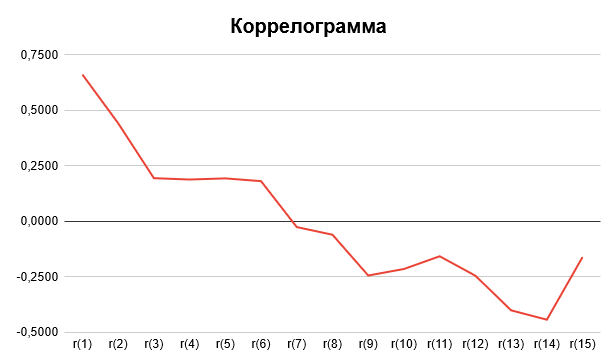
\includegraphics{img/correlogramma.png}
    \caption{Коррелограмма}
\end{figure}
Поскольку коррелограмма АКФ имеет максимум при $k=1 (r(1) = 0,6617)$, то ряд содержит только тенденцию (тренд).
Тренд - это долговременная тенденция изменения исследуемого временного ряда.

\newpage

\mysec{Уравнение тренда}
На основе коррелограммы опишем тренд линейной функцией:
\begin{gather*}
    x(t) = kt + b
\end{gather*}
Для вычисления коэффициентов $k$ и $b$ воспользуемся функцией $\varPhi(k, b) = \sum\limits_{i=1}^n (x_i - kt_i -b)^2$. Для нахождения коэффициентов $k$ и $b$ решим следующую систему уравнений:
\begin{gather*}
    \begin{dcases}
        \der{\varPhi}{k} = 0, \\
        \der{\varPhi}{b} = 0
    \end{dcases}
    \Rightarrow
    \begin{dcases}
        \der{\varPhi}{k} = -2 \sum\limits_{i=1}^n (x_it_i - t_i^2k - t_ib) = 0, \\
        \der{\varPhi}{b} = -2 \sum\limits_{i=1}^n (x_i - kt_i - b) = 0
    \end{dcases}
    \Rightarrow \\
    \begin{dcases}
        k \sum\limits_{i=1}^n t_i^2 + b \sum\limits_{i=1}^n t_i = \sum\limits_{i=1}^n x_it_i, \\
        k \sum\limits_{i=1}^n t_i + nb = \sum\limits_{i=1}^n x_i
    \end{dcases}
    \Rightarrow \\
    \begin{dcases}
        9455k + 465b = 2019386,97, \\
        465k + 30 b = 132262,79 \\
    \end{dcases}
    \Rightarrow \\
    \begin{dcases}
        k\left(9455 - \frac{465^2}{30}\right) = 2019386,97 - \frac{465 \cdot 132262,79}{30}, \\
        b = \frac{132262,79 - 465k}{30}
    \end{dcases}
    \Rightarrow
    \begin{dcases}
        k = -13,65, \\
        b = 4620,39
    \end{dcases}
\end{gather*}
Следовательно, уравнение тренда будет выглядеть следующим образом:
\begin{gather*}
    x(t) = -13,65t + 4620,39
\end{gather*}
\newpage

\mysec{Ошибки тренда}


\end{document}
